\section{A Program-Centered Task Taxonomy}
\label{sec:taxonomy}

The taxonomy determines what is generated, sampled, and analyzed as
one task.  It must therefore distinguish genuine reasoning objectives without
turning every prompt argument or visual style into a new sampling unit. \trace
organizes tasks as follows; Table~\ref{tab:task-boundaries} previews how
the resulting boundary rule treats representative variations.
\begin{equation}
  \text{domain} \longrightarrow \text{scene} \longrightarrow \text{task}.
  \label{eq:public-taxonomy}
\end{equation}
A domain groups related visual inputs for reporting and balancing.  A scene is
a stable visible grammar: its object vocabulary, relations, layout family,
and query-facing scaffold. A task binds that grammar to one objective
contract. This hierarchy describes observable and computational structure,
not the internal organization of a generator.

\subsection{Task identity as a contract}

Let a scene contract be $\mathcal{S}$ and an objective contract be
\begin{equation}
  \mathcal{O} = (P,\mathcal{Y},\mathcal{V}),
\end{equation}
where $P$ is a concrete reasoning program, $\mathcal{Y}$ is the answer schema,
and $\mathcal{V}$ is the verifier contract that specifies answer serialization
and scoring. A task is the pair $T=(\mathcal{S},\mathcal{O})$. The
program must specify the candidate set, operand roles, intermediate
computation, final operator, and output binding; a label such as
``count objects'' or ``select an extremum'' is not by itself a task
definition.

Two candidates can be merged only when
\begin{equation}
  T_i \equiv T_j
  \quad\Longleftrightarrow\quad
  \mathcal{S}_i \simeq \mathcal{S}_j,\;
  P_i \simeq P_j,\;
  \mathcal{Y}_i=\mathcal{Y}_j,\;
  \mathcal{V}_i \simeq \mathcal{V}_j,
  \label{eq:task-equivalence}
\end{equation}
where $\simeq$ permits renaming literal operands, such as a color or category,
but preserves the candidate set, operand arity, intermediate objects, output
binding, visible scaffold, and scoring semantics.  A change to any of these
elements produces a separate task even if the prompts look similar or the
final answer has the same type.

\subsection{Queries are semantic arguments, not task units}

An internal query $q$ selects a bounded argument of $P$ when that argument
meaningfully changes the question while leaving the contract in
Equation~\ref{eq:task-equivalence} intact.  In the boxplot example in
Figure~\ref{fig:taxonomy-boundaries}, largest and smallest IQR are two values
of an extremum-direction argument.  Both branches use the same boxes,
compute $q_3-q_1$, and return a group label under the same verifier contract.
They are therefore queries of one task rather than two tasks.

By contrast, counting icons with one shape attribute and counting icons that
satisfy both a shape and a color are separate objectives.  The latter adds an
operand role and constructs an intersection before counting.  Inclusive OR is
also separate: although it uses the same attributes and returns the same
answer type, its selected set is a union rather than an intersection.  In
geometry, directly applying the exterior-angle relation and solving an
algebraic angle expression likewise remain separate because they construct
different intermediate quantities.  Sharing an integer answer type does not
erase that program difference.

Generation parameters $\theta$ occupy a third category.  Palette, font,
layout, labels, board dimensions, and local difficulty may alter the rendered
instance while leaving the prompt semantics and program unchanged.  The two
cell boards in Figure~\ref{fig:taxonomy-boundaries}, for example, instantiate
the same reachability task under different visual and structural parameters.
Treating these changes as queries would promote incidental generation choices
into the reasoning taxonomy.

\begin{figure*}[t]
  \centering
  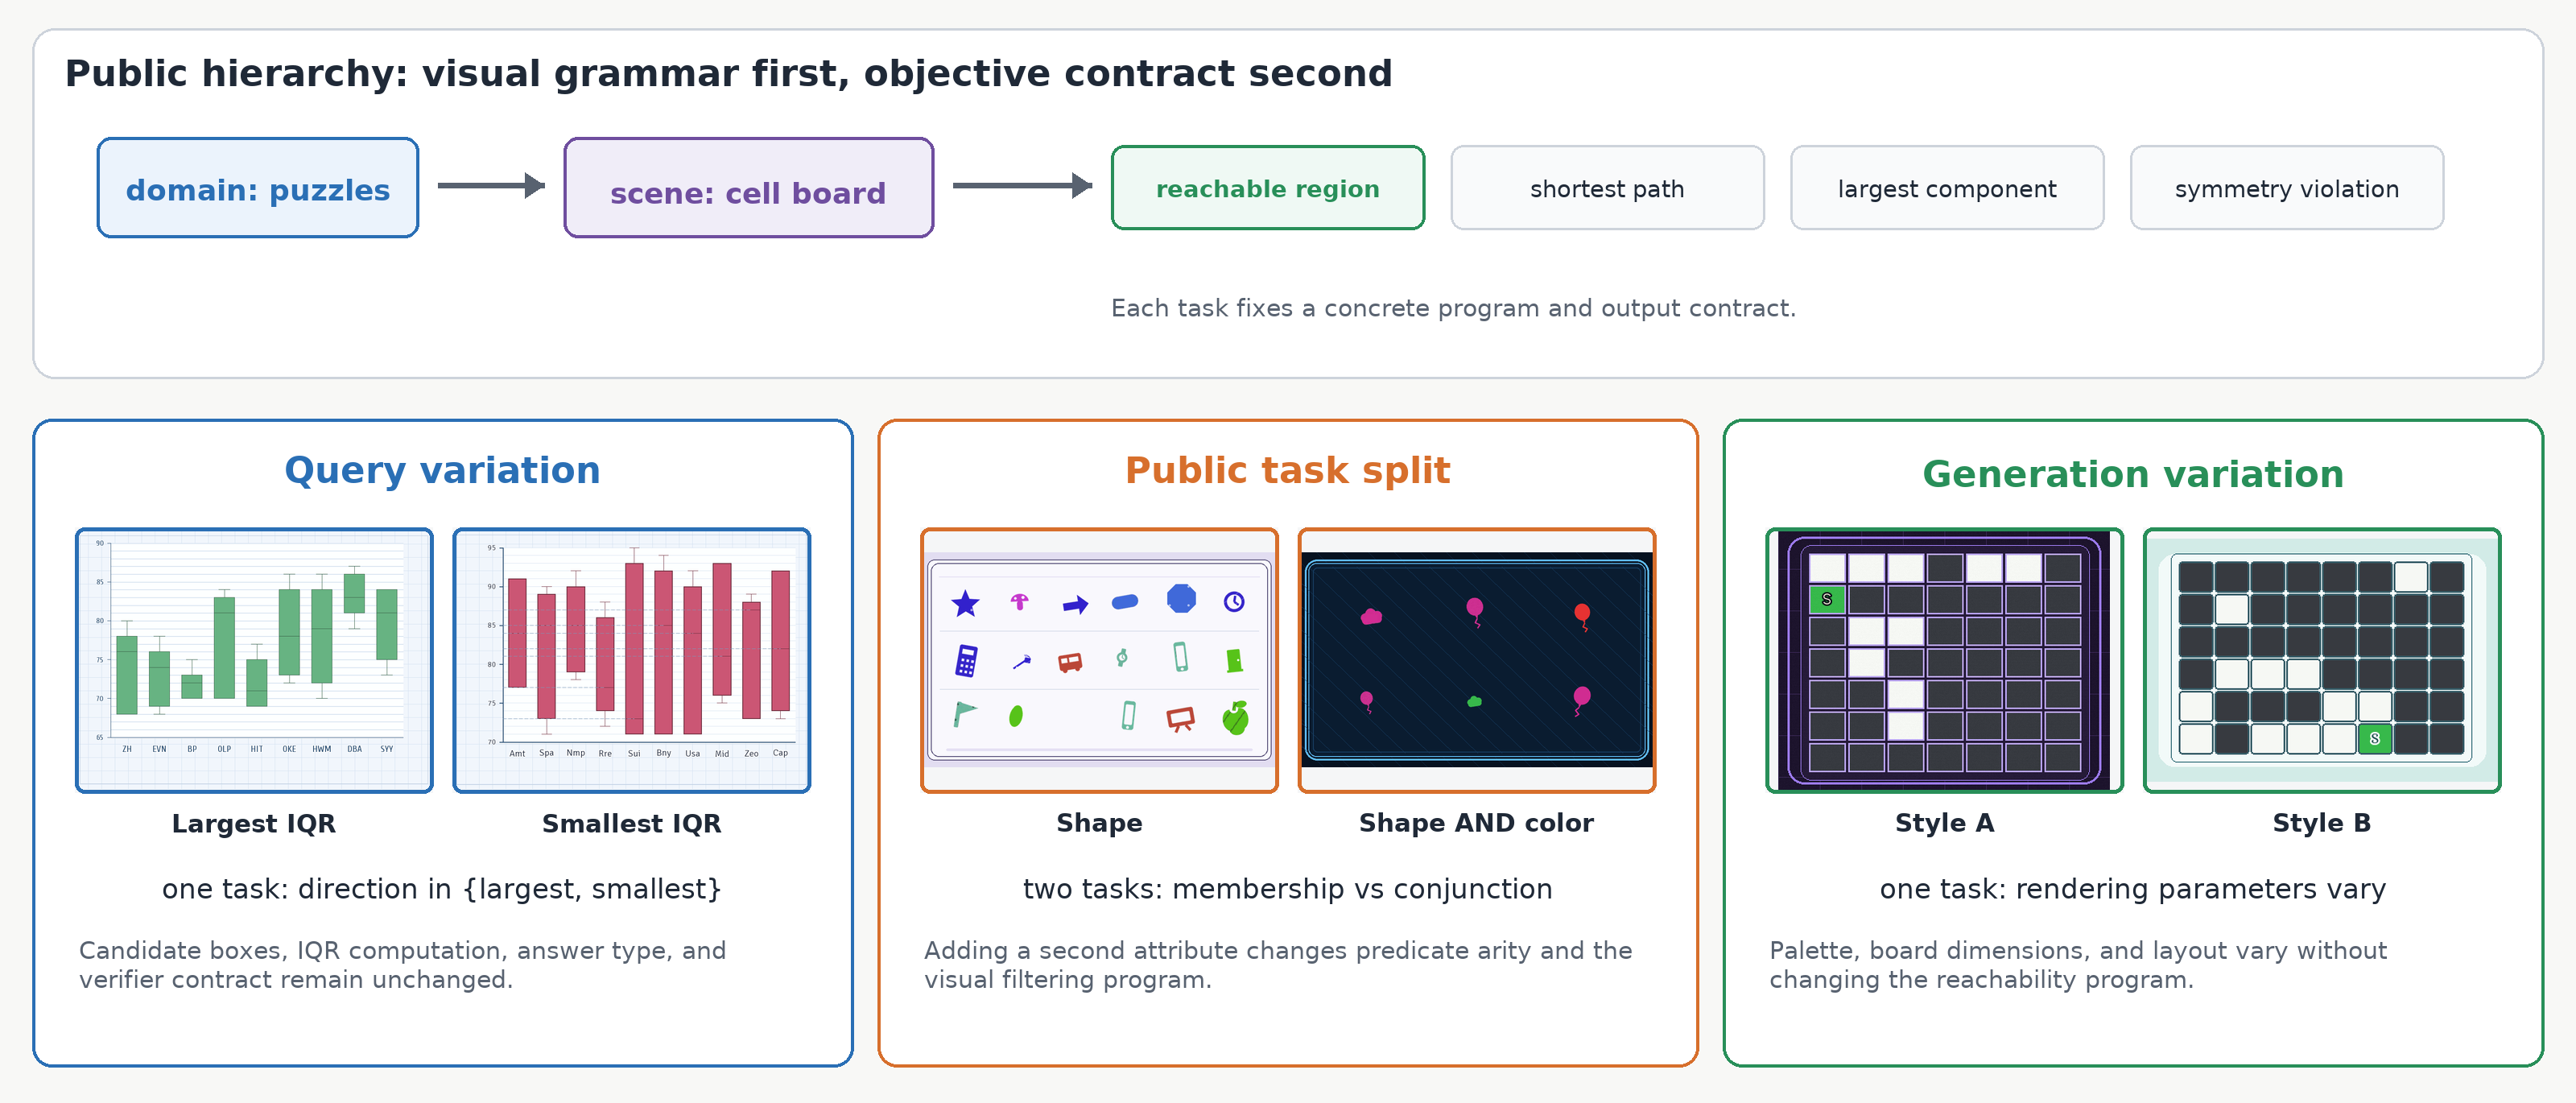
\includegraphics[width=\textwidth]{figures/taxonomy_boundaries.png}
  \caption{Task-boundary examples. The hierarchy first fixes a visual
  scene grammar and then a reasoning objective.  Extremum direction remains a
  query when the boxplot program and output contracts are unchanged (left).
  Adding a conjunctive attribute changes the icon-filtering program and creates
  another task (center).  Rendering and layout variation remain generation
  parameters when the reachability program is unchanged (right).}
  \label{fig:taxonomy-boundaries}
\end{figure*}

\begin{table}[t]
  \centering
  \small
  \caption{Applying the task-boundary rule to representative variations.}
  \label{tab:task-boundaries}
  \begin{tabular}{@{}p{0.30\columnwidth}p{0.47\columnwidth}p{0.17\columnwidth}@{}}
    \toprule
    Variation & Contract effect & Classification \\
    \midrule
    Palette, layout, item count & Program and output roles unchanged & Generation \\
    Largest vs. smallest IQR & Only extremum direction changes & Query \\
    Shape vs. shape-and-color count & Predicate arity and selected set change & New task \\
    AND vs. inclusive OR count & Intermediate set operator changes & New task \\
    Direct vs. algebraic exterior angle & Derivation rule changes & New task \\
    Same extremum family in another scene & Visual grammar or output contract changes & New task \\
    \bottomrule
  \end{tabular}
\end{table}

\subsection{Canonical programs without collapsing scenes}

Program names are canonicalized across the environment so that equivalent
operators can be found and analyzed together.  For example, choosing the
boxplot with extreme IQR and choosing the grid line with an extreme shape count
both instantiate an extreme-metric selection family. They remain separate
tasks because their scene grammars, metric constructions, outputs, and
visible scaffolds differ.  Canonicalization thus normalizes reasoning
vocabulary without discarding the visual contract that defines the task.

The distinction matters statistically. Tasks are sampled uniformly by
default, with query sampling occurring inside a selected task.  Splitting one
program into many operand-specific tasks would give that behavior excess
probability mass, while merging different programs would hide heterogeneous
reasoning behind one average.  We consequently merge only demonstrated
contract equivalences and otherwise preserve the narrower task boundary. The
result is a taxonomy that defines a common unit for generation, supervision,
sampling, and analysis.

\subsection{Compositional extensibility}

The same boundary rule permits controlled growth. A new visual grammar expands
the scene set, while a new reasoning contract expands the tasks available
within a scene. Because visual realization and objective definition are
separate, rendering primitives can be shared or improved without changing the
statistical identity of an existing task. Conversely, one scene can support
several reasoning programs without duplicating its visual construction. This
factorization makes breadth an explicit composition of scene and objective
coverage rather than an accumulation of unrelated templates.
